
\begin{figure}
	\centering
	\subfigure[Ground truth trajectory of Seq.0.]{
		\begin{minipage}[t]{0.4\linewidth}
			\centering
			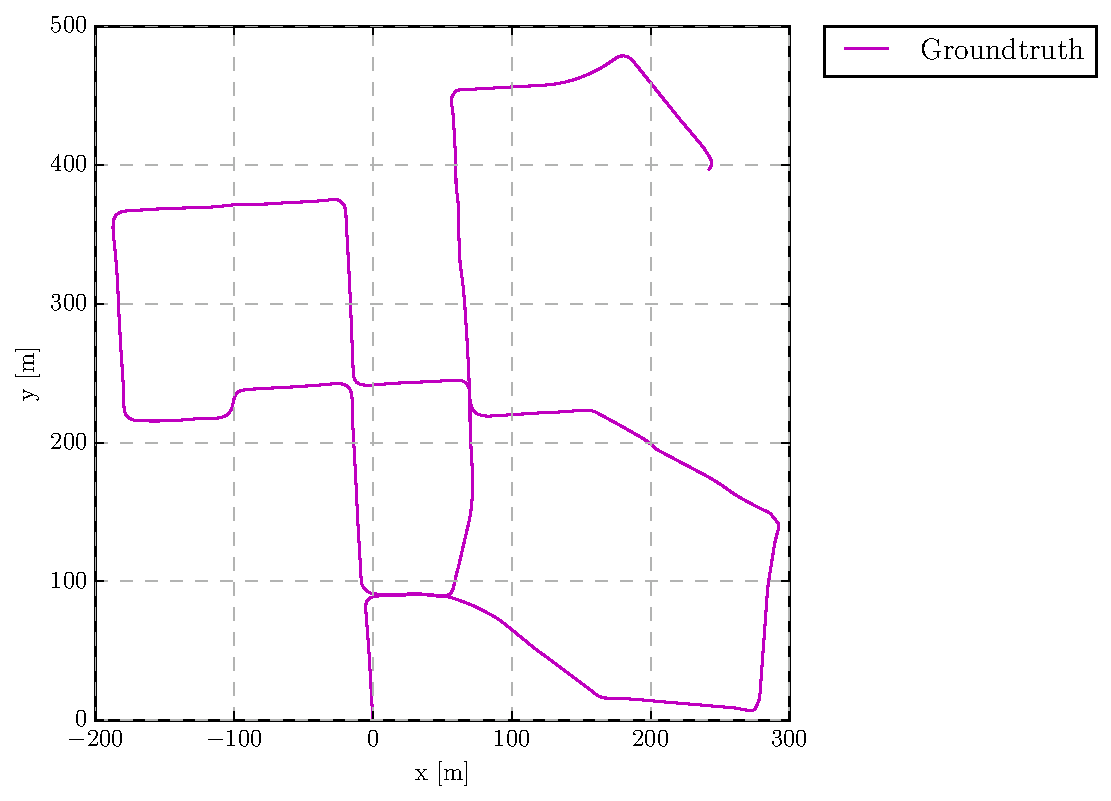
\includegraphics[width=2in]{Chapter4/KITTI/00server/32/plots/trajectory_side_gt_sim3_-1.pdf}
			%\caption{fig1}
		\end{minipage}
	}
	\subfigure[Ground truth trajectory of Seq.1.]{
		\begin{minipage}[t]{0.4\linewidth}
			\centering
			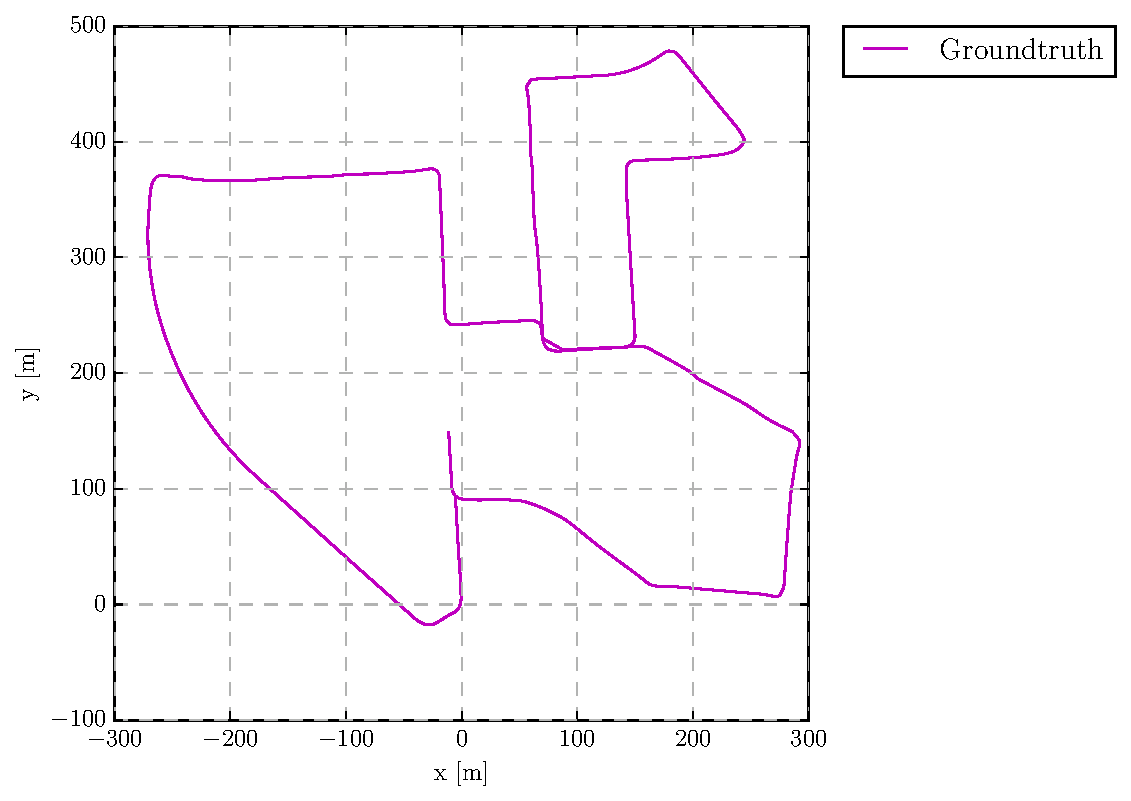
\includegraphics[width=2in]{Chapter4/KITTI/00server/33/plots/trajectory_side_gt_sim3_-1.pdf}
			%\caption{fig2}
		\end{minipage}
	}
	\vfill
	\subfigure[Ground truth trajectory of complete Sequence 00.]{
		\begin{minipage}[t]{\linewidth}
			\centering
			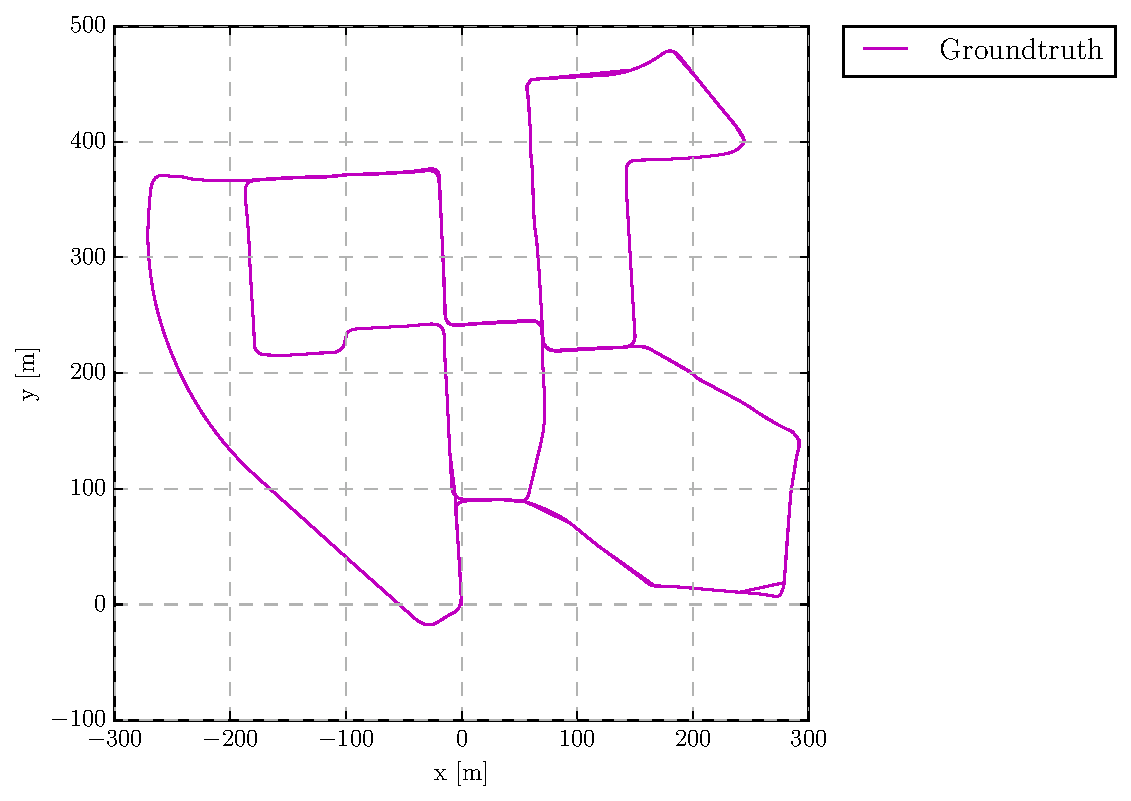
\includegraphics[width=5in]{Chapter4/KITTI/00server/plots/trajectory_side_gt_sim3_-1.pdf}
			%\caption{fig1}
		\end{minipage}
	}
	\caption{Ground truth trajectory of partial and complete sequences of KITTI Datasets.}
	\label{fig:kittigt}
\end{figure}

\begin{figure}
	\centering
	\subfigure[Relative translation error.]{
		\begin{minipage}[t]{0.4\linewidth}
			\centering
			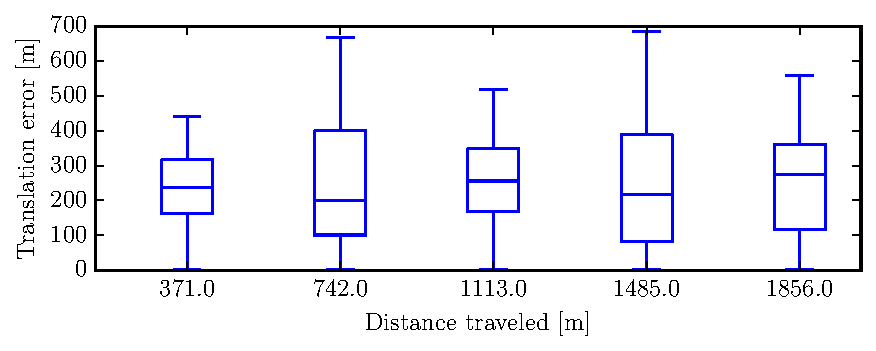
\includegraphics[width=2in]{Chapter4/KITTI/00/gps/plots/rel_translation_error.pdf}
			%\caption{fig1}
		\end{minipage}
	}
	\subfigure[Relative translation error by percent.]{
		\begin{minipage}[t]{0.4\linewidth}
			\centering
			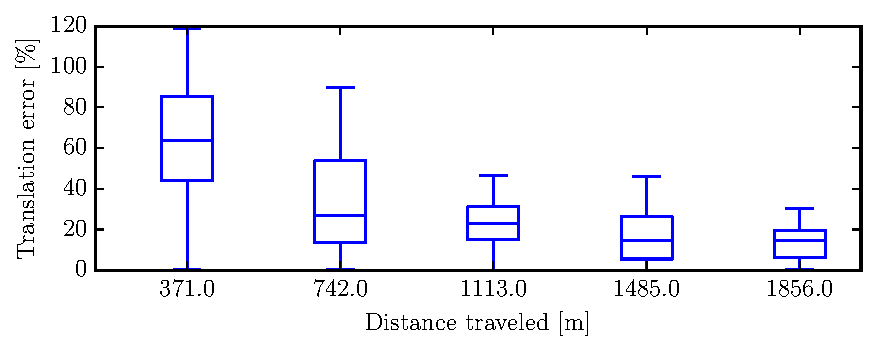
\includegraphics[width=2in]{Chapter4/KITTI/00/gps/plots/rel_translation_error_perc.pdf}
			%\caption{fig2}
		\end{minipage}
	}
	\vfill
	\subfigure[Relative yaw error.]{
		\begin{minipage}[t]{0.4\linewidth}
			\centering
			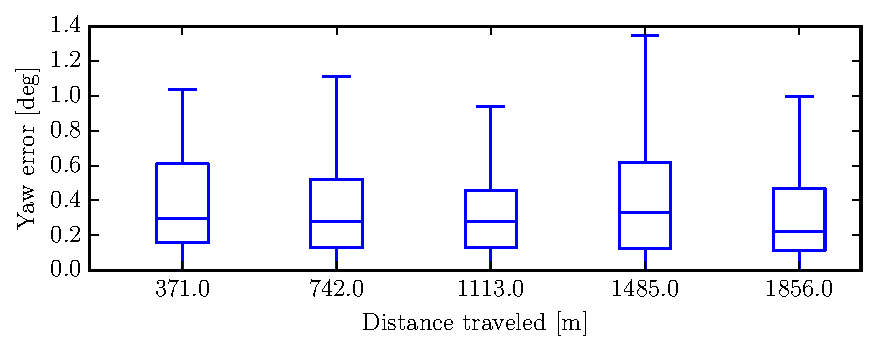
\includegraphics[width=2in]{Chapter4/KITTI/00/gps/plots/rel_yaw_error.pdf}
			%\caption{fig1}
		\end{minipage}
	}
\ifoutputscaleerror
	\subfigure[Scale error.]{
		\begin{minipage}[t]{0.4\linewidth}
			\centering
			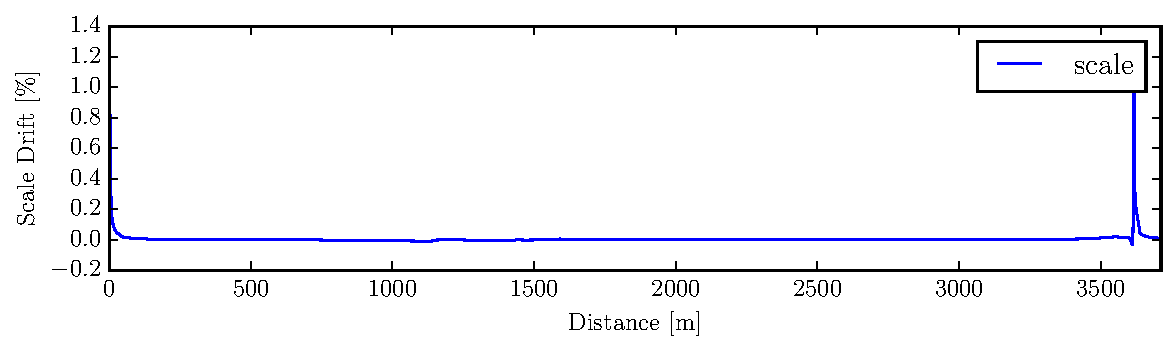
\includegraphics[width=2in]{Chapter4/KITTI/00/gps/plots/scale_error_sim3_-1.pdf}
			%\caption{fig2}
		\end{minipage}
	}
\fi
	\caption{Quantitative evaluation results of CORB-SLAM client mapping the entire KITTI Sequence 00.}
	\label{fig:kittientirequanresult}
\end{figure}

\begin{figure}
	\centering
	\subfigure[Relative translation error.]{
		\begin{minipage}[t]{0.4\linewidth}
			\centering
			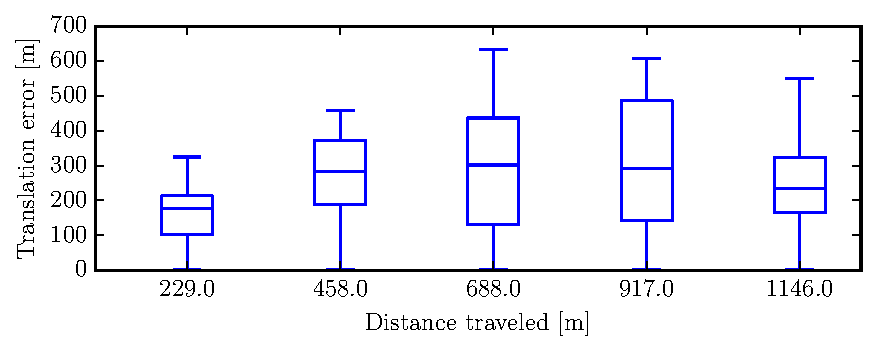
\includegraphics[width=2in]{Chapter4/KITTI/00server/32/plots/rel_translation_error.pdf}
			%\caption{fig1}
		\end{minipage}
	}
	\subfigure[Relative translation error by percent.]{
		\begin{minipage}[t]{0.4\linewidth}
			\centering
			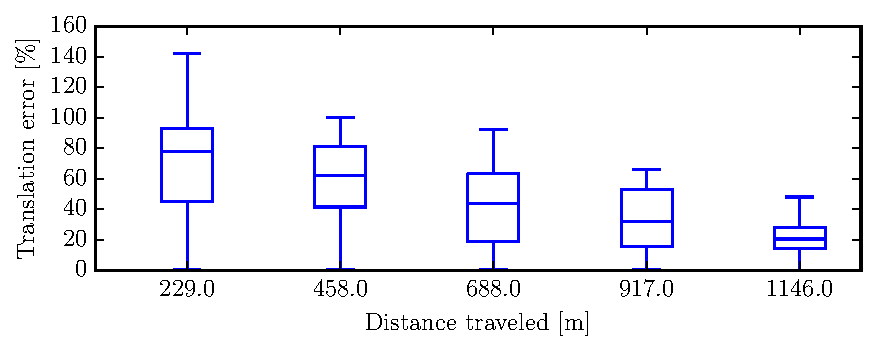
\includegraphics[width=2in]{Chapter4/KITTI/00server/32/plots/rel_translation_error_perc.pdf}
			%\caption{fig2}
		\end{minipage}
	}
	\vfill
	\subfigure[Relative yaw error.]{
		\begin{minipage}[t]{0.4\linewidth}
			\centering
			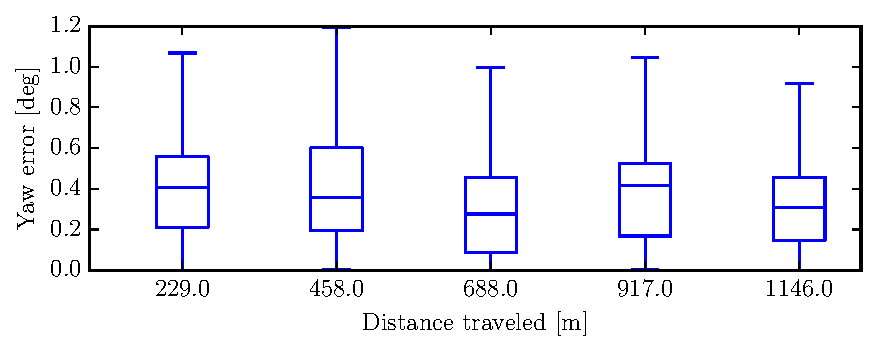
\includegraphics[width=2in]{Chapter4/KITTI/00server/32/plots/rel_yaw_error.pdf}
			%\caption{fig1}
		\end{minipage}
	}
\ifoutputscaleerror
	\subfigure[Scale error.]{
		\begin{minipage}[t]{0.4\linewidth}
			\centering
			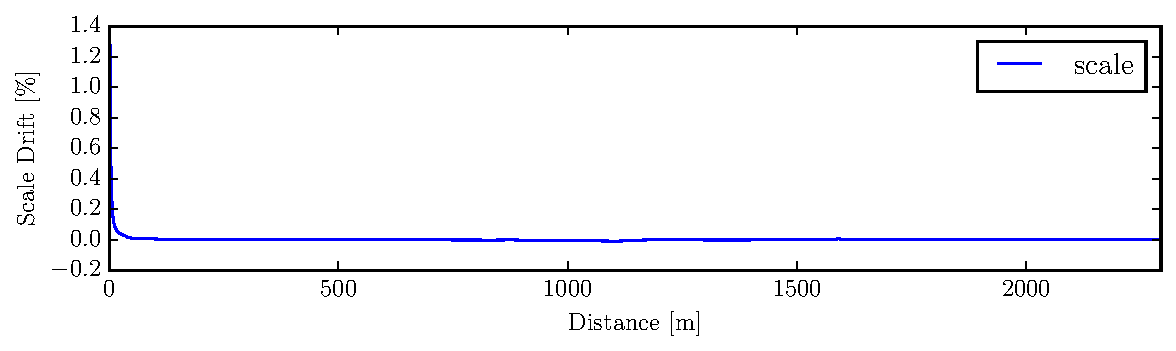
\includegraphics[width=2in]{Chapter4/KITTI/00server/32/plots/scale_error_sim3_-1.pdf}
			%\caption{fig2}
		\end{minipage}
	}
\fi
	\caption{Quantitative evaluation results of CORB-SLAM client mapping  KITTI partial Seq.0.}
	\label{fig:kittiseq0quanresult}
\end{figure}

\begin{figure}
	\centering
	\subfigure[Relative translation error.]{
		\begin{minipage}[t]{0.4\linewidth}
			\centering
			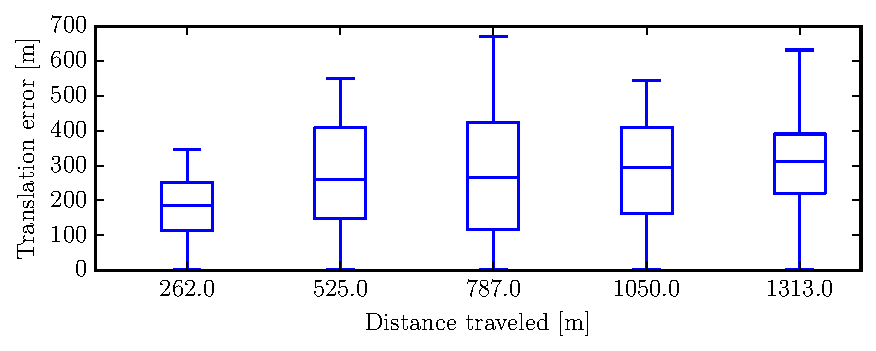
\includegraphics[width=2in]{Chapter4/KITTI/00server/33/plots/rel_translation_error.pdf}
			%\caption{fig1}
		\end{minipage}
	}
	\subfigure[Relative translation error by percent.]{
		\begin{minipage}[t]{0.4\linewidth}
			\centering
			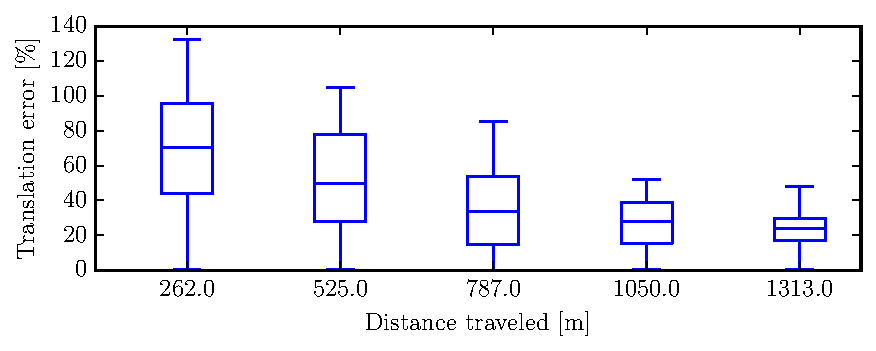
\includegraphics[width=2in]{Chapter4/KITTI/00server/33/plots/rel_translation_error_perc.pdf}
			%\caption{fig2}
		\end{minipage}
	}
	\vfill
	\subfigure[Relative yaw error.]{
		\begin{minipage}[t]{0.4\linewidth}
			\centering
			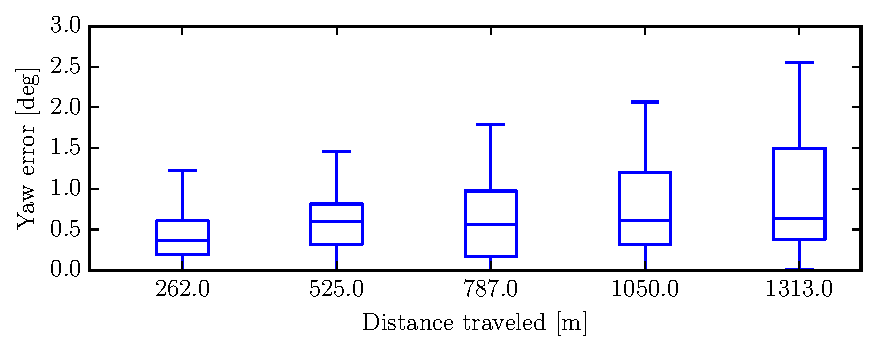
\includegraphics[width=2in]{Chapter4/KITTI/00server/33/plots/rel_yaw_error.pdf}
			%\caption{fig1}
		\end{minipage}
	}
\ifoutputscaleerror
	\subfigure[Scale error.]{
		\begin{minipage}[t]{0.4\linewidth}
			\centering
			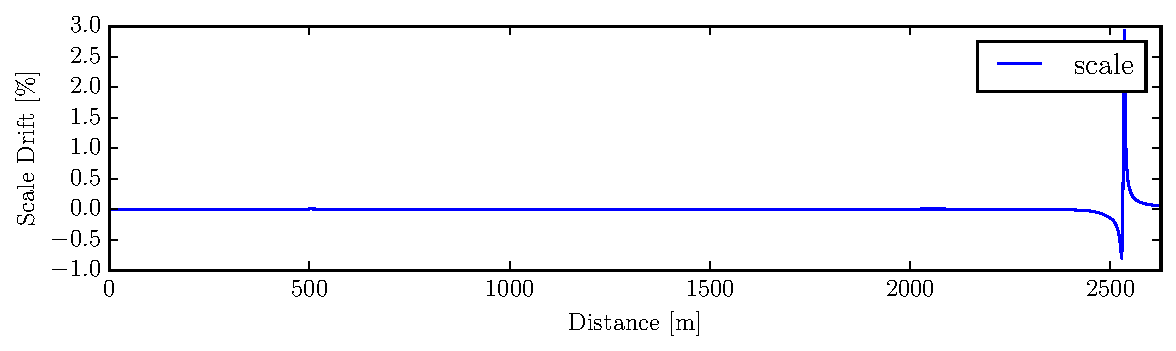
\includegraphics[width=2in]{Chapter4/KITTI/00server/33/plots/scale_error_sim3_-1.pdf}
			%\caption{fig2}
		\end{minipage}
	}
\fi
	\caption{Quantitative evaluation results of CORB-SLAM client mapping  KITTI partial Seq.1.}
	\label{fig:kittiseq1quanresult}
\end{figure}

\begin{table*}
	\centering
	\caption{Quantitative results of mapping unseparated Sequence 00.}
	\begin{threeparttable}
			\ifoutputscaleerror
		\begin{tabular}{|c|c|c|c|c|}
			\hline
			Distance(m)\tnote{1} & Rel. Trans.(m)\tnote{2}  & Rel. Trans.($\%$)\tnote{3} & Rel. Yaw(deg)\tnote{4} & Scale Err.($\%$)\tnote{5}  \\
			\hline
			371& 229.69 & 61.91 & 0.37 & - \\
			\hline
			742&260.10& 35.05 & 0.37 & - \\
			\hline
			1113&260.20& 23.38 & 0.31 & - \\
			\hline
			1485&240.93& 16.22 & 0.40 & - \\
			\hline
			1856&255.16& 13.74 & 0.32 & 0.05\\
			\hline
		\end{tabular}
		\begin{tablenotes}
			\footnotesize
			\item[1] Distance in meter traveled before each time of statistics. 
			\item[2] Mean relative translation error in meter.
			\item[3] Mean relative translation error in percent.
			\item[4] Mean relative yaw error in degree.
			\item[5] Median scale error in percent.
		\end{tablenotes}
	\fi
	
			\begin{tabular}{|c|c|c|c|c|}
		\hline
		Distance(m)\tnote{1} & Rel. Trans.(m)\tnote{2}  & Rel. Trans.($\%$)\tnote{3} & Rel. Yaw(deg)\tnote{4}   \\
		\hline
		371& 229.69 & 61.91 & 0.37  \\
		\hline
		742&260.10& 35.05 & 0.37 \\
		\hline
		1113&260.20& 23.38 & 0.31  \\
		\hline
		1485&240.93& 16.22 & 0.40 \\
		\hline
		1856&255.16& 13.74 & 0.32 \\
		\hline
	\end{tabular}
	\begin{tablenotes}
		\footnotesize
		\item[1] Distance in meter traveled before each time of statistics. 
		\item[2] Mean relative translation error in meter.
		\item[3] Mean relative translation error in percent.
		\item[4] Mean relative yaw error in degree.
	\end{tablenotes}
	\end{threeparttable}
	\label{tbl:kitticlientquanresult}
\end{table*}

\begin{table*}
	\centering
	\caption{Quantitative results of mapping Seq.0.}
	\begin{threeparttable}
		\begin{tabular}{|c|c|c|c|c|}
			\hline
			Distance(m)\tnote{1} & Rel. Trans.(m)\tnote{2}  & Rel. Trans.($\%$)\tnote{3} & Rel. Yaw(deg)\tnote{4}   \\
			\hline
			229& 161.01 & 70.31 & 0.40  \\
			\hline
			458&267.43& 58.38 & 0.42\\
			\hline
			688&299.07& 43.47 & 0.31 \\
			\hline
			917&306.37& 33.41 & 0.39 \\
			\hline
			1146&256.09& 22.35 & 0.34 \\
			\hline
		\end{tabular}
		\begin{tablenotes}
			\footnotesize
			\item[1] Distance in meter traveled before each time of statistics. 
			\item[2] Mean relative translation error in meter.
			\item[3] Mean relative translation error in percent.
			\item[4] Mean relative yaw error in degree.
		\end{tablenotes}
	
	\ifoutputscaleerror
			\begin{tabular}{|c|c|c|c|c|}
		\hline
		Distance(m)\tnote{1} & Rel. Trans.(m)\tnote{2}  & Rel. Trans.($\%$)\tnote{3} & Rel. Yaw(deg)\tnote{4} & Scale Err.($\%$)\tnote{5}  \\
		\hline
		229& 161.01 & 70.31 & 0.40 & - \\
		\hline
		458&267.43& 58.38 & 0.42& - \\
		\hline
		688&299.07& 43.47 & 0.31 & - \\
		\hline
		917&306.37& 33.41 & 0.39& - \\
		\hline
		1146&256.09& 22.35 & 0.34 & $2.47\times10^{-3}$\\
		\hline
	\end{tabular}
	\begin{tablenotes}
		\footnotesize
		\item[1] Distance in meter traveled before each time of statistics. 
		\item[2] Mean relative translation error in meter.
		\item[3] Mean relative translation error in percent.
		\item[4] Mean relative yaw error in degree.
		\item[5] Median scale error in percent.
	\end{tablenotes}
\fi
	\end{threeparttable}
	\label{tbl:kittiseq0quanresult}
\end{table*}

\begin{table*}
	\centering
	\caption{Quantitative results of mapping Seq.1.}
	\begin{threeparttable}
		\begin{tabular}{|c|c|c|c|c|}
			\hline
			Distance(m)\tnote{1} & Rel. Trans.(m)\tnote{2}  & Rel. Trans.($\%$)\tnote{3} & Rel. Yaw(deg)\tnote{4}   \\
			\hline
			262& 229.41 & 114.28 & 0.40  \\
			\hline
			525&412.58& 78.59 & 0.57 \\
			\hline
			787&386.45& 49.10 & 0.61  \\
			\hline
			1050&390.23& 37.16 & 0.77  \\
			\hline
			1313&464.24& 35.36 & 0.89 \\
			\hline
		\end{tabular}
		\begin{tablenotes}
			\footnotesize
			\item[1] Distance in meter traveled before each time of statistics. 
			\item[2] Mean relative translation error in meter.
			\item[3] Mean relative translation error in percent.
			\item[4] Mean relative yaw error in degree.
		\end{tablenotes}
	
	\ifoutputscaleerror
			\begin{tabular}{|c|c|c|c|c|}
		\hline
		Distance(m)\tnote{1} & Rel. Trans.(m)\tnote{2}  & Rel. Trans.($\%$)\tnote{3} & Rel. Yaw(deg)\tnote{4} & Scale Err.($\%$)\tnote{5}  \\
		\hline
		262& 229.41 & 114.28 & 0.40 & - \\
		\hline
		525&412.58& 78.59 & 0.57 & - \\
		\hline
		787&386.45& 49.10 & 0.61 & - \\
		\hline
		1050&390.23& 37.16 & 0.77 & - \\
		\hline
		1313&464.24& 35.36 & 0.89 & 0.21\\
		\hline
	\end{tabular}
	\begin{tablenotes}
		\footnotesize
		\item[1] Distance in meter traveled before each time of statistics. 
		\item[2] Mean relative translation error in meter.
		\item[3] Mean relative translation error in percent.
		\item[4] Mean relative yaw error in degree.
		\item[5] Median scale error in percent.
	\end{tablenotes}
\fi
	\end{threeparttable}
	\label{tbl:kittiseq1quanresult}
\end{table*}

\begin{figure}[H]
	\centering
	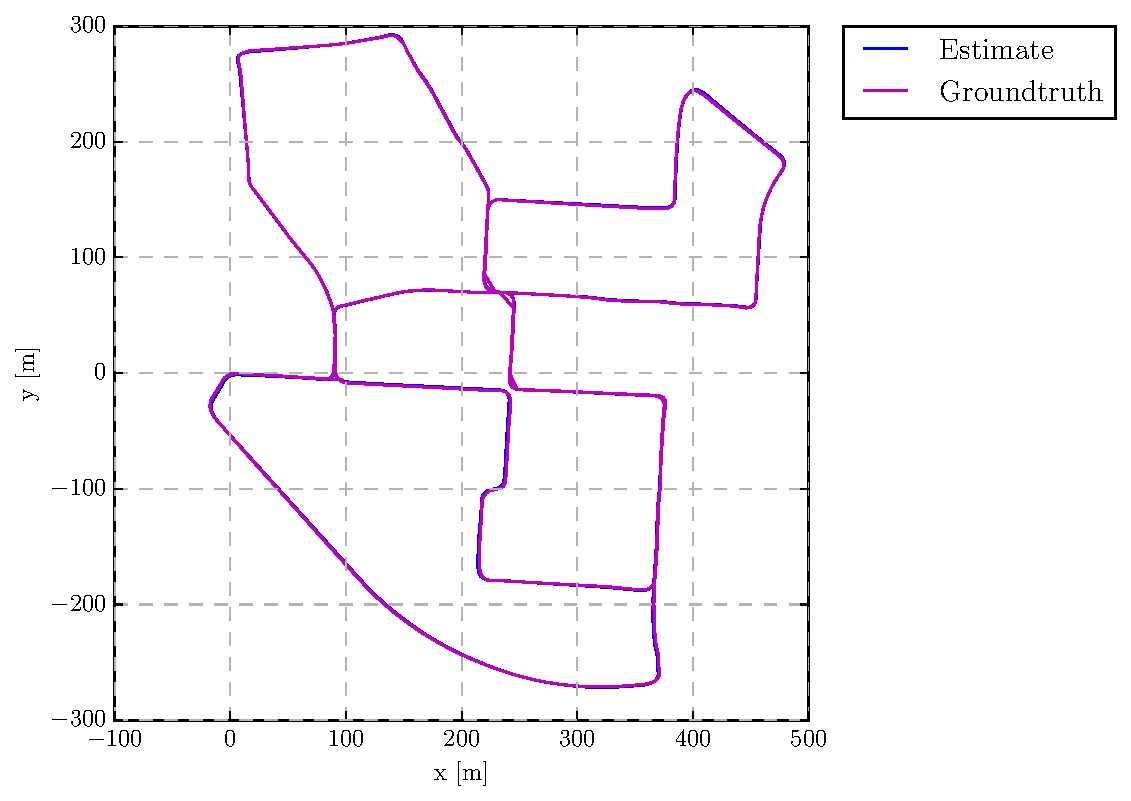
\includegraphics[width=5in]{Chapter4/KITTI/00/gps/plots/trajectory_side_sim3_-1.pdf}
	\caption{Mapping results of the entire sequence without partial sequence.}
	\label{fig:kitticlientmapping} 
\end{figure}

\begin{figure}
	\centering
	\subfigure[Mapping result of Seq.0 compared with ground truth.]{
		\begin{minipage}[t]{0.4\linewidth}
			\centering
			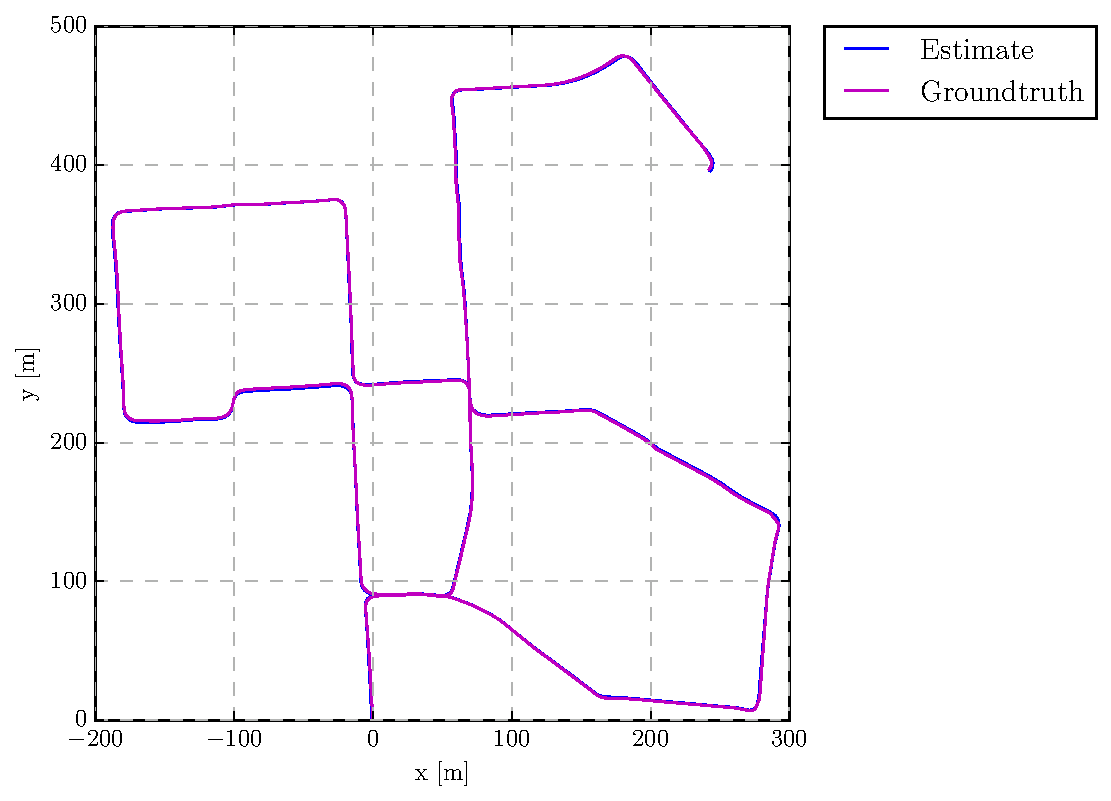
\includegraphics[width=2in]{Chapter4/KITTI/00server/32/plots/trajectory_side_sim3_-1.pdf}
			%\caption{fig1}
		\end{minipage}
	}
	\subfigure[Mapping result of Seq.1 compared with ground truth.]{
		\begin{minipage}[t]{0.4\linewidth}
			\centering
			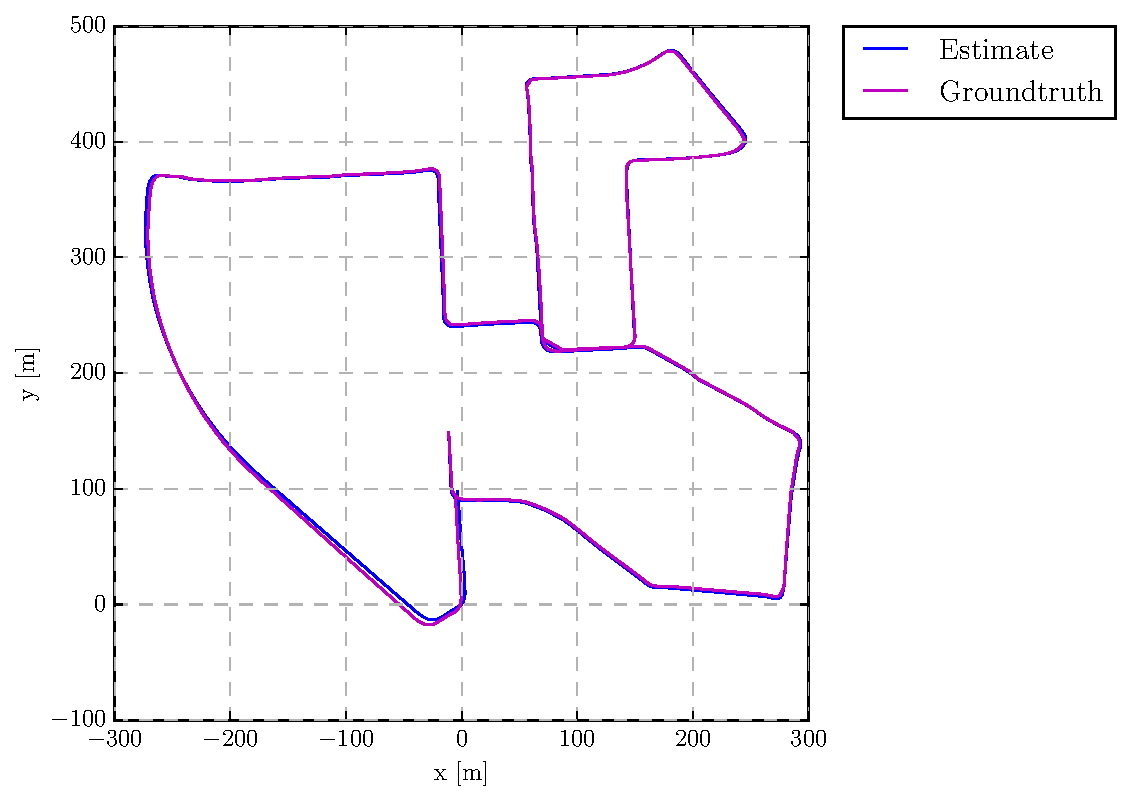
\includegraphics[width=2in]{Chapter4/KITTI/00server/33/plots/trajectory_side_sim3_-1.pdf}
			%\caption{fig2}
		\end{minipage}
	}
	\vfill
	\subfigure[Map Fusion results of Seq.0 and Seq.1 compared with ground truth.]{
		\begin{minipage}[t]{\linewidth}
			\centering
			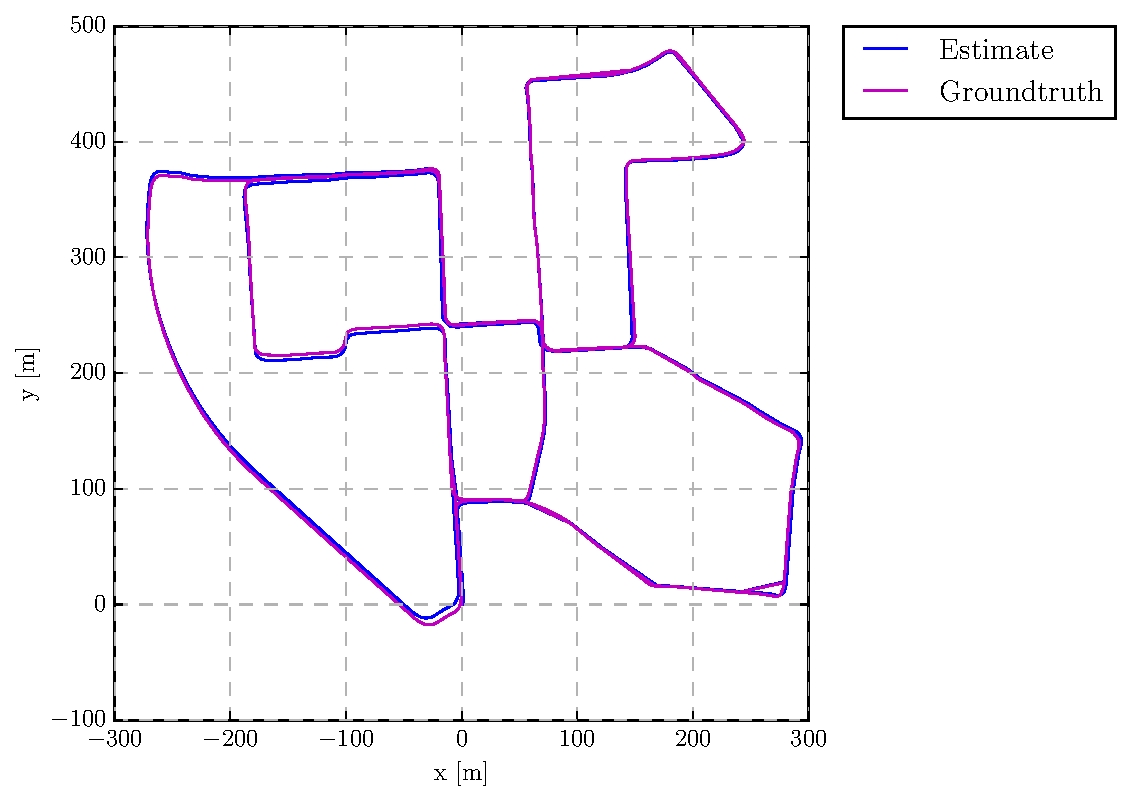
\includegraphics[width=5in]{Chapter4/KITTI/00server/plots/trajectory_side_sim3_-1.pdf}
			%\caption{fig1}
		\end{minipage}
	}
	\caption{Mapping results of Seq.0 and Seq.1, and the map fusion results of KITTI Datasets.}
	\label{fig:kittiresults}
\end{figure}

\begin{figure}
	\centering
	\subfigure[Relative translation error.]{
		\label{sfig:kittireltran}
		\begin{minipage}[t]{0.4\linewidth}
			\centering
			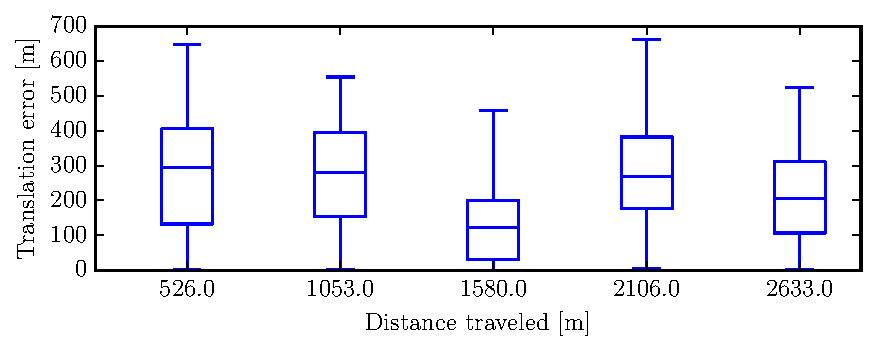
\includegraphics[width=2in]{Chapter4/KITTI/00server/plots/rel_translation_error.pdf}
			%\caption{fig1}
		\end{minipage}
	}
	\subfigure[Relative translation error by percent.]{
		\label{sfig:kittireltranper}
		\begin{minipage}[t]{0.4\linewidth}
			\centering
			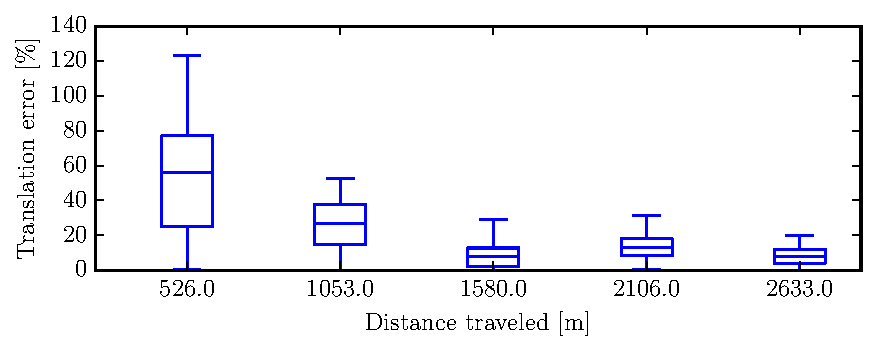
\includegraphics[width=2in]{Chapter4/KITTI/00server/plots/rel_translation_error_perc.pdf}
			%\caption{fig2}
		\end{minipage}
	}
	\vfill
	\subfigure[Relative yaw error.]{
		\label{sfig:kittirelyaw}
		\begin{minipage}[t]{0.4\linewidth}
			\centering
			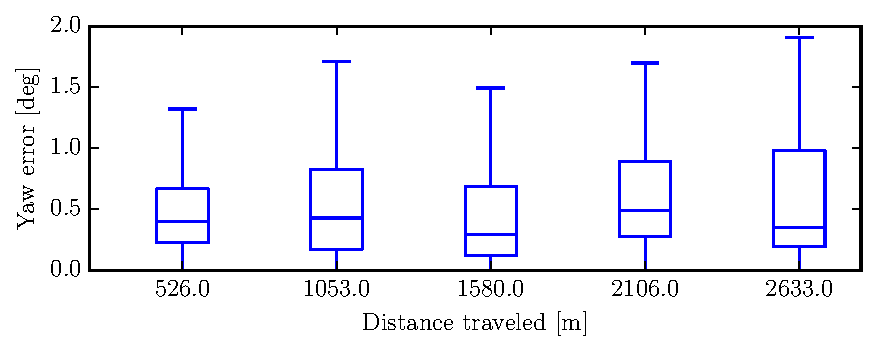
\includegraphics[width=2in]{Chapter4/KITTI/00server/plots/rel_yaw_error.pdf}
			%\caption{fig1}
		\end{minipage}
	}
\ifoutputscaleerror
	\subfigure[Scale error.]{
		\label{sfig:kittiscaleerr}
		\begin{minipage}[t]{0.4\linewidth}
			\centering
			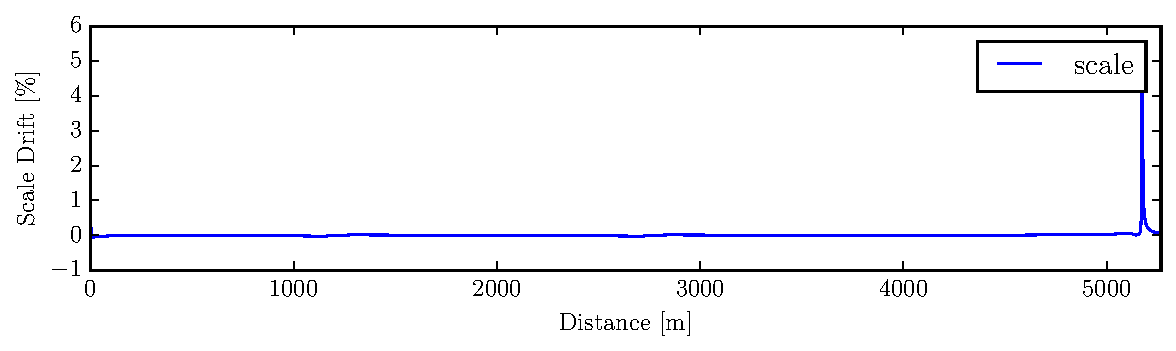
\includegraphics[width=2in]{Chapter4/KITTI/00server/plots/scale_error_sim3_-1.pdf}
			%\caption{fig2}
		\end{minipage}
	}
\fi
	\caption{Quantitative evaluation results of fused map of KITTI Datasets.}
	\label{fig:kittiquanresult}
\end{figure}

\begin{table*}
	\centering
	\caption{Quantitative results of map fusion evaluation on KITTI partial sequences.}
	\begin{threeparttable}
	\ifoutputscaleerror
	\begin{tabular}{|c|c|c|c|c|}
		\hline
		Distance(m)\tnote{1} & Rel. Trans.(m)\tnote{2}  & Rel. Trans.($\%$)\tnote{3} & Rel. Yaw(deg)\tnote{4} & Scale Err.($\%$)\tnote{5}  \\
		\hline
		526& 283.40 & 53.88 & 0.46& - \\
		\hline
		1053&276.16& 26.23 & 0.51 & - \\
		\hline
		1580&153.74& 9.73 & 0.48 & - \\
		\hline
		2106&284.95& 13.53 & 0.57 & - \\
		\hline
		2633&219.66& 8.34 & 0.54 & -0.15\\
		\hline
	\end{tabular}
      \begin{tablenotes}
		\footnotesize
		\item[1] Distance in meter traveled before each time of statistics. 
		\item[2] Mean relative translation error in meter.
		\item[3] Mean relative translation error in percent.
		\item[4] Mean relative yaw error in degree.
		\item[5] Median scale error in percent.
	\end{tablenotes}
\fi

	\begin{tabular}{|c|c|c|c|c|}
	\hline
	Distance(m)\tnote{1} & Rel. Trans.(m)\tnote{2}  & Rel. Trans.($\%$)\tnote{3} & Rel. Yaw(deg)\tnote{4} \\
	\hline
	526& 283.40 & 53.88 & 0.46 \\
	\hline
	1053&276.16& 26.23 & 0.51  \\
	\hline
	1580&153.74& 9.73 & 0.48  \\
	\hline
	2106&284.95& 13.53 & 0.57  \\
	\hline
	2633&219.66& 8.34 & 0.54 \\
	\hline
\end{tabular}
\begin{tablenotes}
	\footnotesize
	\item[1] Distance in meter traveled before each time of statistics. 
	\item[2] Mean relative translation error in meter.
	\item[3] Mean relative translation error in percent.
	\item[4] Mean relative yaw error in degree.
\end{tablenotes}


	\end{threeparttable}
	\label{tbl:kittiquanresult}
\end{table*}